\documentclass[12pt]{article}

\usepackage[spanish]{babel}
\usepackage[utf8]{inputenc}
\usepackage{graphicx}
\usepackage{geometry}
\usepackage{verbatim}
\usepackage{xcolor}
\usepackage{fancyhdr}
\usepackage{lastpage}
\usepackage{pdfpages}
\usepackage{listings}
\usepackage{schemata}

\geometry{top=25mm,left=15mm,right=15mm,a4paper}

\pagestyle{fancy}
\fancyhf{}
\lhead{Computación Concurrente}
\cfoot{Página \thepage\ de \pageref{LastPage}}

\graphicspath{./}

\begin{document}
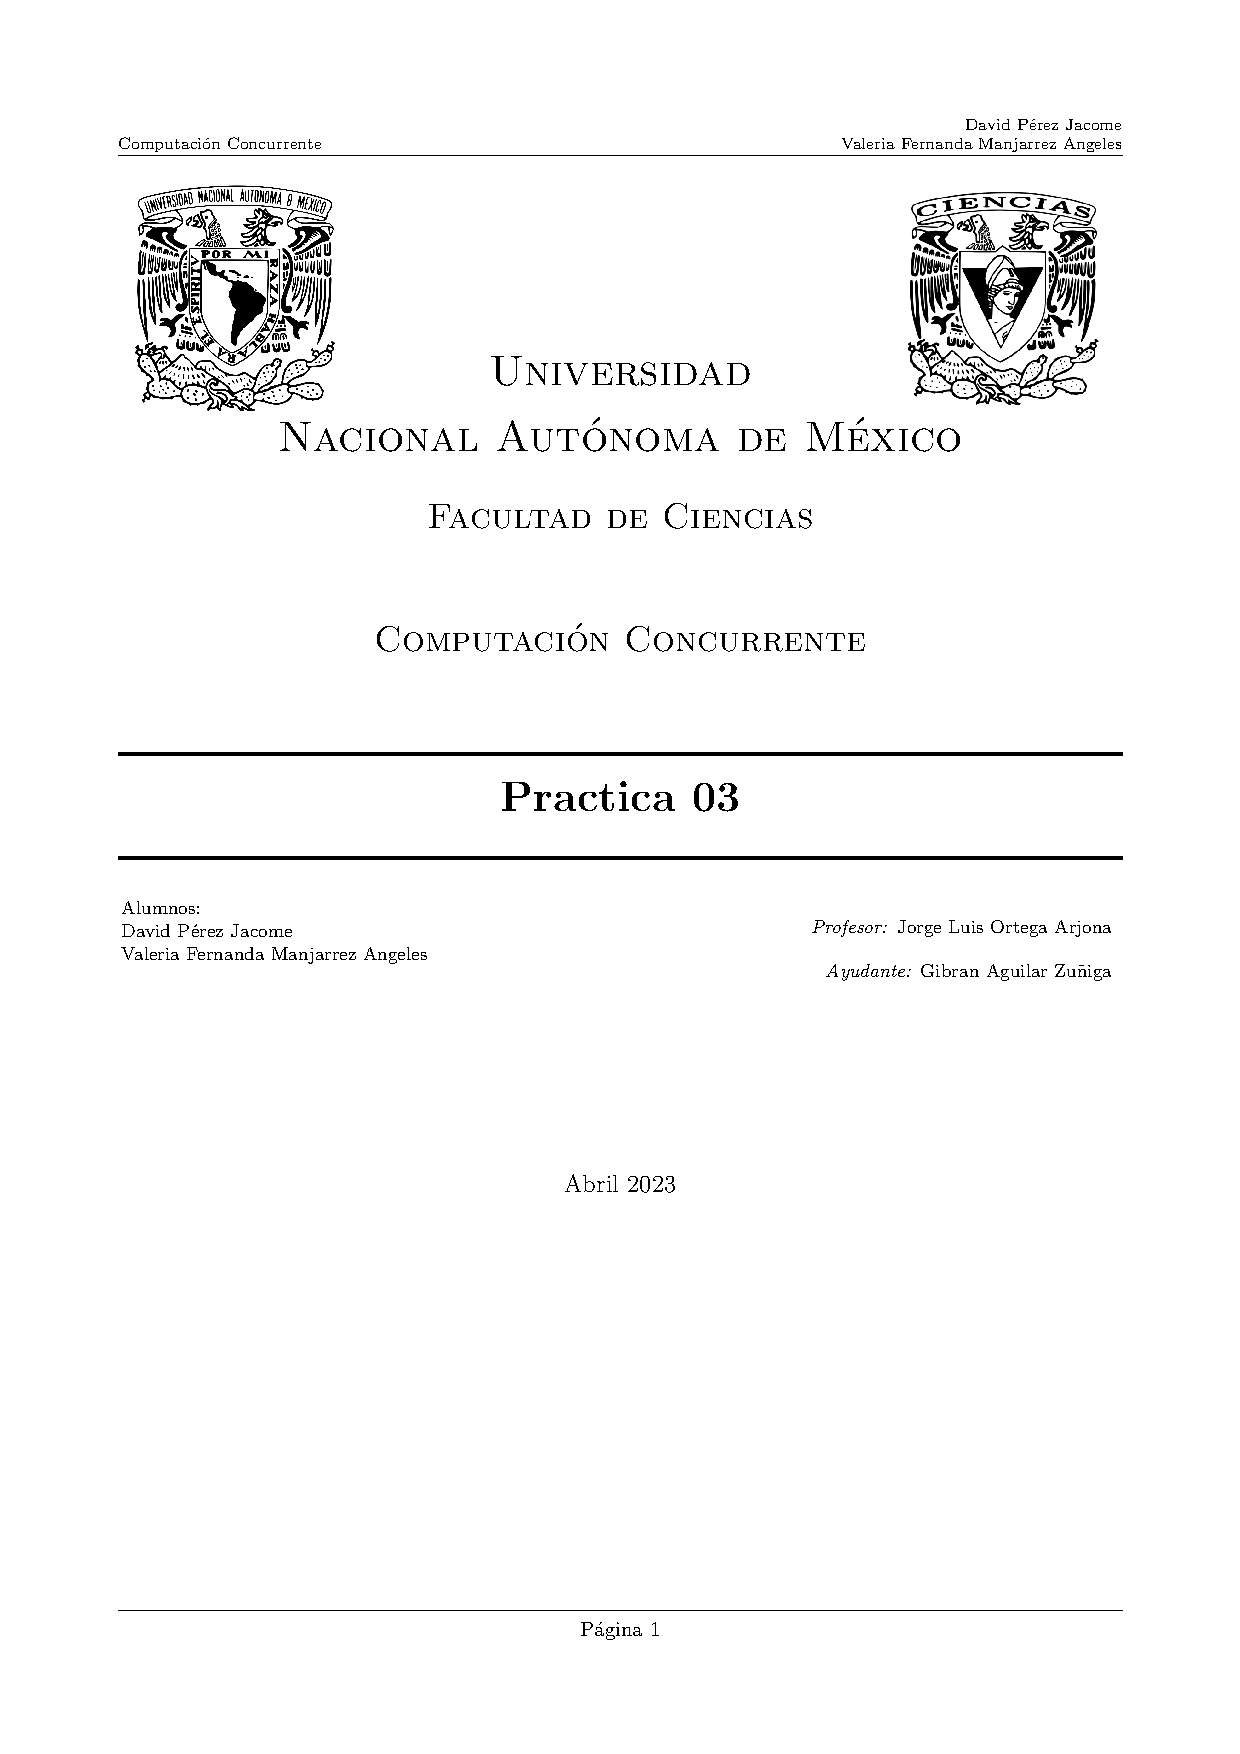
\includepdf{Portada.pdf}
{\color{red} \section*{\textbf{PRACTICA 03}}}
\vspace{1em}

{\color{blue} \subsection*{\textbf{Preguntas:}}}


Deberán detallar a profundidad las respuestas y en caso de ser necesario hacer diagramas 
para ejemplificar tu respuesta.\\


\begin{enumerate}
    \item ¿Qué es un monitor? (2 puntos).
    \vspace{2mm}
    
    \textbf{Respuesta.}
    \item ¿Qué es un proceso distribuido? (2 puntos).
    \vspace{2mm}
    
    \textbf{Respuesta.}
    \item ¿Cúales son las diferencias entre Computo Concurrente y Computo Paralelo? (2 puntos).
    \vspace{2mm}
    
    \textbf{Respuesta}
    \item Haz un TDA de monitores (4 puntos).
    \vspace{2mm}
    
    \textbf{TDA para monitores:}\\
    \begin{verbatim}
        / Declaración del TDA de semáforos
        
TDA_Monitor:

    
    \end{verbatim}\\
\end{enumerate}

{\color{blue} \subsection*{\textbf{Ejecución:}}}

Para ejecutar nuestro programa es necesario:\\

\begin{enumerate}
    \item Localizarnos en en directorio: \textbf{Practica03}.
    \item Ejecutamos: \textbf{mvn compile}
    \item Ejecutamos el ejecutable que se localiza en el directorio target: \textbf{java -jar target/Practica01.jar}. 
\end{enumerate}
\end{document}